\documentclass[11pt]{article}
\usepackage[utf8]{inputenc}
\usepackage{tikz}
\usepackage{amsmath,amsfonts,amsthm}
\usepackage[vlined, ruled]{algorithm2e}
\usepackage{geometry}
\usepackage[noend]{algpseudocode}
\usetikzlibrary{bayesnet}
\usepackage[nottoc,numbib]{tocbibind}
\usepackage{enumitem,kantlipsum}
\usepackage{float}
\usepackage{titlesec}
\usepackage{natbib}
\usepackage{apalike}
\setcounter{secnumdepth}{4}

\titleformat{\paragraph}
{\normalfont\normalsize\bfseries}{\theparagraph}{1em}{}
\titlespacing*{\paragraph}
{0pt}{3.25ex plus 1ex minus .2ex}{1.5ex plus .2ex}

\setlength{\parskip}{1em}
\geometry{letterpaper,left=1.5in,right=1in,top=1in,bottom=1in}
\setlength\parindent{0pt}
\linespread{1.5}
\newcommand{\E}{\mathrm{E}}
\newcommand{\Var}{\mathrm{Var}}
\newcommand{\N}{\mathcal{N}}
\newcommand{\tr}{tr}

\begin{document}
\pagenumbering{gobble}
{\centering
  \textbf{A Gaussian Approach to Recovering Dynamic Brain Functional Connectivities}\par
  A Thesis\par
  Submitted to the Faculty\par
  in partial fulfillment of the requirements for the\par
  degree of\par
  Master of Science\par
  in\par
  Computer Science\par
  by\par
  Hao Chang\par
  DARTMOUTH COLLEGE\par
  Hanover, New Hampshire\par
  May, 2017\par
}
\vspace{5mm}
\setlength{\parskip}{0em}
\begin{flushright}
Examining Committee:\par
\vspace{5mm}
$\rule{5cm}{0.15mm}$\par
Hany Farid\par
\vspace{5mm}
$\rule{5cm}{0.15mm}$\par
Qiang Liu\par
\vspace{5mm}
$\rule{5cm}{0.25mm}$\par
Jeremy Manning\par
\end{flushright}
\setlength{\parskip}{1em}
\newpage


\null\par
\newpage
\pagenumbering{roman}
\section{Abstract}
Recent research focused on the analysis of brain functional connectivities---pair-wise correlation between time series of activities in different brain regions---has achieved monumental breakthroughs in improving our understanding of the human brain. Moreover, new efforts have attempted to cast functional connectivities as dynamic processes that change from moment to moment and have revealed that important brain dynamics information exists within these correlation structures. A tried and tested method of recovering dynamic brain functional connectivities is the sliding window method, which applies the correlation function on a window of time points to calculate the temporal correlation at the window center. However, this process is essentially finding the average correlation of all the time points within the sliding window instead of the actual temporal correlation at the window center, and thus provides only a low resolution representation of the temporal ground truth. In addition, the sliding window approach requires an extended buffer to calculate the correlation at each time point. Therefore it is unable to recover the dynamic correlations at the edges of the time series, resulting in substantial data loss. In order to more effectively recover dynamic functional connectivities from brain data, we present the Time Sequence Correlation Recovery (TimeCorr) method. TimeCorr calculates the correlation at each time point $t$ by multiplying the correlation components of the whole time series by a Gaussian distribution centering at $t$. The use of Gaussian coefficients increases the temporal resolution of TimeCorr calculations by putting more emphasis on the time points near the Gaussian center. At the same time, TimeCorr is able to improve the stability of its results by incorporating information from the entire dataset into each of its calculations. Lastly, using a flexible Gaussian distribution instead of a stiff window makes it possible for TimeCorr to calculate the dynamic correlations of time points at the edges of the time series. To illustrate the effectiveness of TimeCorr, we compare its performance with that of the sliding window approach, and show that TimeCorr produces similar and often times more accurate and stable results in all of our test cases.

\newpage
\section{Acknowledgements}
Firstly, I would like to thank my mentors Professor Jeremy Manning of the Psychological and Brain Sciences Department at Dartmouth College and Professor Qiang Liu of the Computer Science Department at Dartmouth College. Professor Manning and Professor Liu were great inspirations for me throughout this project. Their deep understanding of their respective fields and constant flow of bright ideas expanded my understanding of what it means to love and excel at what I want to do. Professor Manning and Professor Liu provided timely guidance whenever I was in need and constantly encouraged me to try out new ideas and reach for higher standards.

Secondly, I would like to thank Professor Hany Farid of the Computer Science Department at Dartmouth College. Professor Farid kindled my first spark of interest in Computer Science and pushed me to pursue graduate education at Dartmouth. He has been a role model for me throughout my time at Dartmouth and will always be an inspiration for me in my future pursuits in life.

Thirdly, I would like to thank Andy Heusser and Kirsten Ziman in the Contextual Dynamics Laboratory in the Neuroscience Department at Dartmouth College. Andy and Kirsten played crucial roles in helping me overcome my lack of experience in neuroscience related research. Their patient and timely assistance helped me through many difficulties at crucial stages of my research.

Fourthly, I would like to thank Dilin Wang, Jun Han and Yihao Feng in the DartML Laboratory in the Computer Science Department at Dartmouth College. Their door were always open whenever I ran into a difficult spot or had questions about my research or writing.

Finally, I must express my very profound gratitude to my parents for providing me with unfailing support and continuous encouragement throughout my years of study and through the process of researching and writing this thesis. This accomplishment would not have been possible without them. Thank you.

\newpage
\tableofcontents
\newpage
\listoffigures
\newpage
\pagenumbering{arabic}

\section{Introduction}
Human beings have an insatiable desire to understand---not only the things around us, but also ourselves. Why do we behave and respond the way we do \citep{hasson2012}? How do we learn and adapt \citep{hasson2004,hasson2005}? What do we believe or value \citep{Greene01}? How does social context affect the way we think \citep{Matthew2015}? These questions have mesmerized wise men and women for thousands of years, but the answers continue to evade us. For many, the key to understanding human behavior lies in our brain, the central hub of all of our thoughts and decision making. So, when a new technology emerged and allowed us to study the brain in a quantitative manner, it opened a door of endless possibilities for those who possesses an aptitude for quantitative analysis and a hunger to learn more about our own identity.

Functional Magnetic Resonance Imaging, often referred to as fMRI, was first discovered and applied as a brain mapping method in 1990 by Seiji Ogawa \citep{Ogawa90}. This technology then quickly popularized among Brain Science related research due to its unprecedented low health risk to subjects and its ability to accurately translate brain activities into highly-structured quantitative data \citep{Logothetis01,Friston99,Friston98}. Once abstract brain activities are converted into signs and digits, exploring patterns in the brain simply devolves into intricate mathematical problems. For example, by treating each brain fMRI image as a feature vector, Machine Learning algorithms trained on a subset of the data can learn to identify cognitive patterns (e.g., which part of a movie someone is watching) and extract similar patterns from held-out brain images \citep{Norman06,peterson12,peterson17}. These applications typically treat each brain image in isolation, and attempt to decode patterns of activities associated with each of several candidate brain states. However, important stimulus-driven activities in fMRI data are often obscured by noise created by non stimulus-driven neural activities \citep{peterson11}, which greatly reduces the effectiveness of any effort to analyze relevant brain activities \citep{hasson2009}. To address this issue, new branches of research have been emerging that specifically focus on the extraction of useful information from noisy brain fMRI data by conducting a time series analysis incorporating information from the entire dataset \citep{tang2017}, and one of the most fruitful directions involves analyzing functional connectivities within the brain \citep{peterson19} \citep{peterson20}.

The brain can be divided in various ways---according to different rules of systemization (by functionality, organization, activity patterns, etc)---into a set of regions, and functional connectivity describes the correlation between the time series of activations each pair of brain regions exhibits. When we observe the brain, the neural activities can appear incredibly complex. But the mechanics of the brain are far from random, rather, the correlation patterns our brains exhibit are highly structured. Presumably, this mirrors the complex but highly structured nature of our internal thoughts and experiences. Many past studies on functional connectivity have focused on using resting state data (fMRI images taken as participants rest in the scanner with their eyes open) to estimate a single correlation matrix for each person, which provides a rich database for mapping the relations among brain processes and their contributions to perception, action and cognition \citep{peterson9,Bassett2017}. The cognitive information of each subject was then used as identifiers to compare how the relationship between brain activities and task behaviors differ or agree between subjects \citep{Turke13,Rubinov2010,peterson10}.

Recent research efforts have revealed that important cognitive information is also contained in the temporal correlational structure of time series brain activities \citep{davidson2016}. As a result, approaches focusing on understanding the brain through analysis of dynamic brain functional connectivities begun to rapidly emerge \citep{Nigam2016,Hutchinson2013}. One of the most significant advancements comes from a recent paper by Uri Hasson's group, which casts functional connectivity as a dynamic process that changes from moment to moment depending on the specific stimulus of that moment \citep{hasson2016}. When analyzing the dynamic functional connectivities of one experimental subject in isolation, one can examine how (or whether) the correlational structure of these activity patterns (across a given set of brain regions) varies according to the cognitive task the subject is performing. The paper also presents the revolutionary Inter-Subject Functional Correlation (ISFC) analysis, which cross-examines functional connectivities across multiple subjects to isolate stimulus-dependent inter-regional correlations from noise created by random neural activities. The Contextual Dynamics Lab successfully applied dynamic functional connectivity and ISFC analyses in their most recent paper on Hierarchical Topographic Factor Analysis (HTFA), and demonstrated that functional connectivity patterns and basic brain activation patterns contain partially non-overlapping information on stimulus-driven brain dynamics \citep{jeremy2017}.

Although functional connectivity analyses of brain data has evolved significantly \citep{olaf2005,khambhati2017}, the method for calculating dynamic functional connectivities in most research is still the sliding window method, where the correlation function is applied on the brain activations of time points within a window of set length to calculate the functional connectivity at the central time point. To calculate the functional connectivities of following time points, the window is shift forward one time point at a time until the edge of the window reaches the end of the time series \citep{enrico2011,elena2012}. However, the sliding window method possesses three fundamental limitations:

Firstly, \textbf{the sliding window approach causes significant data loss.} As the sliding window approach requires an extended buffer around each time point to calculate its functional connectivity, it is unable to conduct calculations near each end of the time series. Therefore, when a sliding window setup with a window length of $L_w$ is applied on a dataset with $t$ time points, it can only retrieve the functional connectivities of $n=t-l+1$ time points, thereby losing important information on $l-1$ time points.

Secondly, \textbf{the sliding window approach only provides low resolution representation of the temporal ground truth.} As the sliding window approach directly applies the correlation function on a time window centering around the time point of interest, it is actually calculating the average functional connectivity over all time points within the time window. This averaging process provides only a low resolution representation (rough estimation) of temporal ground truth (the actual functional connectivity at each time point), which may be insufficient for moment-by-moment dynamic functional connectivity analysis.

Thirdly, \textbf{the sliding window approach lacks flexibility.} When a sliding window setup with a window length of $L_w$ is used to calculate the functional connectivities of a time series, there is loss of information for $L_w-1$ time points. Therefore, in order to retain functional connectivity information for a sufficient number of time points for further analysis, the sliding window length is restricted to a small range of values. As the performance of sliding window implementations with different window lengths varies greatly on datasets with different dynamic correlation structures, this restriction places great limitations on the recovery capabilities of the sliding window approach. In many situations, sliding window implementations with insufficient window length provide only a poor approximation of the true moment-by-moment dynamic correlation patterns.

To address these problems, we present TimeCorr, a lossless and more flexible method for functional connectivity calculation that finds its inspiration directly from the fundamental correlation function. Like the sliding window method, TimeCorr is able to recover functional connectivity from fMRI brain images with similar if not higher accuracy. But TimeCorr goes beyond the sliding window method by (a) not requiring buffers for its calculations, thereby avoiding data loss, (b) offering extra stability by using all time points in the time series for functional connectivity calculation at every time point, (c) and providing the option to balance the locality and stability of its results through adjusting its temporal resolution parameter.

To achieve the functionalities mentioned above, TimeCorr makes use of the Gaussian distribution. By attaching a Gaussian coefficient to components at each time point in the time series, TimeCorr is able to control the amount of influence each neighboring time point has on the calculation of the correlation at the Guassian center. As the Gaussian center (highest density/coefficient) is always at the time point of interest, TimeCorr guarantees to return highly accurate approximations of the temporal ground truth. In addition, the user can choose to have more stability in the results by choosing coefficients from a Gaussian distribution with a larger variance; or higher temporal resolution and more locality by choosing coefficients from a distribution with a lower variance. In the Results section, we demonstrate the effectiveness of the TimeCorr approach through comprehensive testing and evaluation on synthetic datasets with a variety of dynamic correlation structures.

In addition, we were also curious if the advantages of TimeCorr will allow us to discovery new functional connectivity patterns in real brain fMRI datasets that have been heretofore inaccessible by the sliding window method. Since we lack knowledge of the true functional connectivity structures of real fMRI datasets, we present the TimeCorr Decoding Analysis as new means to assessing the quality of our recovery efforts. To evaluate the quality of dynamic functional connectivity recovery at each time point in a time series, the TimeCorr Decoding Analysis finds the moment-by-moment correlation between corresponding time points in the ISFC of two random equal divisions of the subject data. Time points that share high similarity across all subjects have low probability of containing noise and high probability of being correctly recovered and stimulus-driven, therefore the TimeCorr Decoding Analysis gives a good evaluation of the amount of useful information contained in the recovered dynamic functional connectivity at each time point in the time series. We are interested in how the TimeCorr Decoding Analysis results vary across dynamic functional connectivities recoveried using different TimeCorr and sliding window implementations from real fMRI datasets. The results are shown and discussed in more detail in the Results section.

\newpage
\section{Model Description}
\subsection{Single Subject TimeCorr}
The TimeCorr method was designed for the purpose of replacing the sliding window method as a lossless alternative to achieve more accurate calculations of dynamic functional connectivities (the temporal correlation at each time point between pairs of brain regions) from brain fMRI data. The sliding window method operates by applying the correlation calculation function on the activations of time points within a window of length $L_w$ and centering on the time point of interest $t$, where $L_w$ must be of considerable magnitude for the sliding window method to achieve respectable accuracy. However, due to its inherent design flaw, using the sliding window method on a dataset of time length $T$ could only yield functional connectivities for $T-L_w+1$ data points, a loss not insignificant due to the typical magnitude of $L_w$. In addition, as the sliding window method places equal weights on every time point within its window of calculation, it can only achieve a rough approximation of the average correlation within the window but not the instantaneous truth at each time point.

To solve these problems, we designed the TimeCorr method, which finds inspiration from the fundamental correlation function. Instead of isolating only a block of time points, TimeCorr effectively utilizes information from the entire dataset for functional connectivity calculation at every time point. To ensure temporal accuracy in TimeCorr's results, the components at each time point are multiplied by a weight drawn from a normalized Gaussian density function so that the influence of each time point on the calculation of functional connectivity at time point $t$ is proportional to its distance from $t$. When we observe the correlation function:
\begin{align*}
C(x,y) = \frac{\sum_{t=1}^T (x_t-\bar{x})(y_t-\bar{y})}{Ts_xs_y},
\end{align*}
the component $(x_t-\bar{x})(y_t-\bar{y})$ represents the temporal relationship between variable $x$ and variable $y$ at time point $t$. Through the application of Gaussian density coefficients, TimeCorr calculations place heavier weights on the relationship components of time points closer to the Gaussian center (the time point of interest) and lighter weights on time points further away. In comparison with the flat averaging in the sliding window approach, this adaptation provides a better representation of the dynamic correlation structure at the time point of interest (the temporal ground truth), while also taking into consideration the general dynamics throughout the entire time series. In addition, this adaptation of the correlation function effectively eliminates the need to sacrifice buffer time points at the beginning and end of the time series, thereby increasing the number of output time points to equal to the number of input time points and avoiding any data loss.

\large{\textbf{Formal Definition}}

\normalsize
Given a single subject's brain activation matrix with $T$ time points and $V$ voxels, to apply TimeCorr:

\begin{enumerate}
\item Base on the amount of influence neighboring time points should have on the functional connectivity calculation at each time point, choose an appropriate Gaussian variance $\sigma$ to generate coefficients.

\item For each time point $t$:
\begin{enumerate}
\item Using a Gaussian density function of variance $\sigma$ and mean $t$, generate an array of coefficients $w_t$ for $T$ time points, where each element $w_x$ of $w_t$ can be calculated through the following equation:
\begin{align*}
w_x = \mathcal{N}(x|t,\sigma) = \frac{1}{\sqrt{2\sigma\pi}}e^{-\frac12 \frac{(x-t)^2}{\sigma}},
\end{align*}
where $\mathcal{N}(x|t,\sigma)$ represents the Gaussian probability density of $x$ when mean is $t$ and variance is $\sigma$.

\item For each voxel $i$, element-wise multiply its activation time sequence $a_i$ by the coefficients array centered at $t$ to create a weighted activations array $S^i_t$.

\item Compute the temporal correlation between voxel $i$ and voxel $j$ at time point $t$ through the equation:

\begin{align*}
R(S^i_t,S^j_t) = \frac{1}{Z}\frac{\sum_{l=0}^T (S_l^i - \bar{S^i_t})\cdot(S^j_l - \bar{S^j_t})\cdot \mathcal{N}(l|t,\sigma)}{s_t^i \cdot s_t^j},
\end{align*}
where
\begin{align*}
\mathcal{N}(l|t,\sigma) &= \frac{1}{\sqrt{2\sigma\pi}}e^{-\frac12 \frac{(l-t)^2}{\sigma}}\\
Z &= \sum_{l=0}^T \mathcal{N}(l|t,\sigma)\\
\bar{S^i_t} &=\frac{1}{Z} \sum_{l=0}^T S^i_l \cdot \mathcal{N}(l|t,\sigma)\\
s_t^i &=\sqrt{ \frac{1}{Z}\sum_{l=0}^T (S_l^i-\bar{S_t^i})^2 \cdot \mathcal{N}(l|t,\sigma)}.\\
\end{align*}
\item Repeat the process above for every voxel pair to create a correlation matrix for time point $t$.
\end{enumerate}
\item Convert the correlation matrix at every time point to its inverse squareform format (a 1-dimensional array containing only the upper right half of the non-diagonal elements of a square matrix), outputting an array of size $T$ by $(V^2-V)/2$ dimensional matrix, where $T$ and $V$ represent the time length and voxel count of the dataset.
\end{enumerate}

The Gaussian variance parameter $V$ gives the user extra freedom to customize the desired level of resolution for temporal correlation calculation. If a large variance is chosen, the influence of neighboring time points on the functional connectivity calculation at each time point is increased, thereby adding smoothness and stability to the resulting functional connectivity time sequence and providing a more accurate representation of the general dynamics. But if a small variance is chosen, most of the weight will be placed on the time point of interest and its immediate neighbors, so the resulting functional connectivity time sequence will have more emphasis on temporal accuracy. After experimenting with different setups, we discovered that choosing a Gaussian variance equal to the minimum between 1000 and the total number of time points achieves a good balance between locality and fluidity. This finding will be discussed in more detail in the Results section.

\subsection{TimeCorr Inter-Subject Functional Connectivity}

Inter-Subject Functional Connectivity (ISFC) is the functional connectivity between brain regions of different subjects \citep{jeremy2017,hasson2016}. The patterns recovered by ISFC is analogous to single subject functional connectivities (which reflect the correlational structure across brain regions within one individual's
brain), but they should reflect only activities that are specifically stimulus-driven. For every subject, we compare its brain activations time sequence with the average activations of all other subjects. Through the process of averaging the activations of multiple subjects, we dampen random noise and emphasize activities that are common across all subjects, which are usually stimulus-dependent. Therefore, when we calculate the functional connectivity matrix between subject activation and the average response from the rest of the participants, the functional connectivities we calculate are more likely to reflect activities that are stimulus-driven.

Furthermore, after we obtain the functional connectivity matrix between each subject and the average of their counterparts, we use Fisher Z-transformation to average the results from all the subjects. In addition to the noise-dampening and stimulus-enhancing effects that comes with averaging, we are also able to gain an unbiased view of the overall stimulus-driven functional connectivity patterns across all subjects within our analysis. The Fisher Z-transformation is applied in the averaging process as a means to stabilize and reduce approximation variance and return a less biased result than that of directly averaging correlations.

\large{\textbf{Formal Definition}}

\normalsize
Given an activations dataset containing $N$ subjects, each with $T$ time points and $V$ voxels, to apply TimeCorr ISFC:
\begin{enumerate}
\item Determine the desired temporal resolution for calculation and select $\sigma$, the variance of the Gaussian density function for TimeCorr coefficients generation.
\item For each subject $s$,
\begin{enumerate}
\item Find the average activation of all other subjects:
\begin{align*}
O_s=\frac{\sum_{i\neq s}^N S_i}{N-1},
\end{align*}
where $S_i$ represents the activation matrix for subject $i$, and $N$ represents the total number of subjects.
\item Find the functional connectivity between the brain activations time series $S$ for subject $s$ and the average activations of all other subjects $O$ using TimeCorr ISFC with variance $\sigma$. The correlation between $S^i_t$---activation of voxel i for subject $s$ at time $t$---and $O^j_t$---average activation of voxel $j$ of all other subjects at time points $t$---is obtained through the following equation:
\begin{align*}
C(S^i_t,O^j_t) = \frac{1}{Z}\frac{\sum_{l=0}^T (S_l^i - \bar{S^i_t})\cdot(O^j_l - \bar{O^j_t})\cdot \mathcal{N}(l|t,\sigma)}{s_t^i \cdot o_t^j},
\end{align*}
where
\begin{align*}
\mathcal{N}(l|t,\sigma) &= \frac{1}{\sqrt{2\sigma\pi}}e^{-\frac12 \frac{(l-t)^2}{\sigma}}\\
Z &= \sum_{l=0}^T \mathcal{N}(l|t,\sigma)\\
\bar{S^i_t} &=\frac{1}{Z} \sum_{l=0}^T S^i_l \cdot \mathcal{N}(l|t,\sigma)\\
\bar{O^j_t} &=\frac{1}{Z} \sum_{l=0}^T O^j_l \cdot \mathcal{N}(l|t,\sigma)\\
s_t^i &=\sqrt{ \frac{1}{Z}\sum_{l=0}^T (S_l^i-\bar{S_t^i})^2 \cdot \mathcal{N}(l|t,\sigma)}\\
o_t^j &=\sqrt{ \frac{1}{Z}\sum_{l=0}^T (O_l^j-\bar{O_t^j})^2 \cdot \mathcal{N}(l|t,\sigma)}.\\
\end{align*}
\item Repeat the above process for every pair of voxels, for every time point to obtain a time series of correlation matrices.
\end{enumerate}
\item Element-wise apply Fisher Z-transformation $F(x)$ to the correlation matrices for each subject at each time point to obtain the corresponding Z-correlation matrices:
\begin{align*}
F(r) = \frac{1}{2}\ln\left(\frac{1+r}{1-r}\right).
\end{align*}
\item Element-wise average the Z-correlation matrices across all subjects:
\begin{align*}
S_Z = \frac{1}{N}\sum^N_{i=1}Z_i.
\end{align*}
\item Element-wise apply inverse Z-transformation $I(x)$ to the average Z-correlation matrix to obtain the TimeCorr ISFC matrix:
\begin{align*}
\text{TimeCorr ISFC} = I(S_Z) = \frac{e^{(S_Z+S_Z^T)}-1}{e^{(S_Z+S_Z^T)}+1}.
\end{align*}
\item Convert the correlation matrix at every time point to its inverse squareform format, and output a $T$ by $(V^2-V)/2$ dimensional matrix containing the average functional connectivity of all subjects in the dataset, where $T$ and $V$ represent the time length and voxel count of the dataset, respectively.
\end{enumerate}

\subsection{Multi-Subject TimeCorr Decoding Analysis}
The Multi-Subject Resampling Analysis is a two-step process designed to evaluate the quality of recovery of stimulus-dependent dynamic functional connectivities from an fMRI dataset. In the first step, we conduct decoding analysis on the dataset by calculating the Multi-Subject TimeCorr ISFC of two random equal divisions of the subject data, and using the results from one group as an estimation of the ground truth (the true moment-by-moment dynamic functional connectivities of the dataset) to evaluate the quality of recovery of each time point in the other other group. Through the process of averaging in the calculation of ISFC of each group, non stimulus-driven neural activities are dampened and activities that are common across subjects are emphasized, thereby increasing the salience of patterns that reflect activities that are only stimulus-driven. Next, we calculate the correlation between the dynamic functional connectivities of each time point in the ``ground truth" with the dynamic functional connectivities of the corresponding time point in the other group. When the correlation between the same time point in both sub-groups is high, it indicates that the average brain activities in one group demonstrates very high similarity with the average brain activities of all subjects in the other group at that time point. When the brain activities of multiple subjects display high similarity for certain time points in their brain activations time sequence, then intuitively there is a high probability that their brain responses for those time points are uniformly caused by their common stimulus. Using this logic, the decoding correlation of the time series helps us visualize the quality of recovery of each time point.

Furthermore, we understand that having more smoothing in the calculation of dynamic functional connectivity (averaging in TimeCorr and the sliding window method) may also result in higher correlation between activations at the same time point across groups. In the most extreme case where the variance of TimeCorr is equal to infinity, which is equivalent to a sliding window with window length equal to the dataset time length, the recovered dynamic functional connectivity will be identical for every time point in the time series, giving us identical correlation across all the time points. To compensate for this, we came up with the second part of the TimeCorr Decoding Analysis: the Resampling Analysis.

The idea behind this analysis is that, if there is too much smoothing in the ISFC matrices (e.g., in the extreme case where every time point has the same functional connectivity), then the original time series will not always have higher correlation than a reshuffled time series. By calculating the proportion of times where a reshuffled time series gives similar or higher correlation than the original time series, we get the resampling accuracy.  Using this parameter, we can correct for the effect of smoothing in our decoding accuracy, and achieve a more realistic understanding of how well the dynamic correlation structure is being recovered.

\large{\textbf{Formal Definition}}

\normalsize
Given a multi-subject dataset containing $S$ subjects, each possessing $T$ time points and $V$ voxels:
\begin{enumerate}
\item Decoding Analysis:
\begin{enumerate}
\item Select a Gaussian variance $\sigma$ for TimeCorr coefficient generation.
\item Randomly divide the subjects into two equal groups.
\item Calculate Inter-Subject Functional Connectivity (ISFC) for each group using TimeCorr. The resulting ISFC matrices are labelled $I_1$ and $I_2$. We arbitrarily designate $I_1$ as a rough estimation of the ground truth.
\item Calculate correlation between the ISFC at each time point in $I_1$ and the ISFC for the corresponding time point in $I_2$, resulting in a decoding correlation array of length $T$.
\item Using the decoding correlation array, we can visualize how well the dynamic functional connectivity at each time point has been recovered. Higher correlation represents a higher probability that the dynamic functional connectivities at a time point is correctly recovered.
\end{enumerate}
\item Resampling Analysis:
\begin{enumerate}
\item Calculate the mean of the decoding correlation array, and label as $C$.
\item For $N$ repetitions:
\begin{enumerate}
\item Roll the time series in $I_2$ forward so that the last time point in the time series becomes the first time point. This reshuffled time series will be labelled $I_{\text{reshuffled}}$.
\item Calculate the mean of the correlation between each time point in $I_1$ and the corresponding time point in $I_{\text{reshuffled}}$, and label as $C_{\text{reshuffled}}$.
\item A repetition is correctly decoded if $C$ is greater than $C_{\text{reshuffled}}$.
\item Set $I_{\text{reshuffled}}$ as the new $I_2$ to be used in the next resampling cycle.
\end{enumerate}
\item Count and record the number of repetitions that were correctly decoded, and label as $N_{\text{correct}}$.
\item Divide $N_{\text{correct}}$ by the total number of repetitions $N$ to get the resampling accuracy of the multi-subject dataset:
\begin{align*}
\text{Resampling Accuracy} = \frac{N_{\text{correct}}}{N}.
\end{align*}
\item Conduct a statistical test to show that the mean decoding correlation of the original time series $C$ is reliably above chance. The p-value can be calculated using the equation:
\begin{align*}
\text{p-value} = 1-\text{Resampling Accuracy},
\end{align*}
and should take a value less than $0.05$ for $95\%$ confidence in our results.
\end{enumerate}
\end{enumerate}

The Multi-Subject TimeCorr Decoding Analysis defined above gives an accurate evaluation of which time points in the time series:

\begin{enumerate}
\item contain dynamic functional connectivities that are likely to be accurate representations of the ground truth.
\item contain dynamic functional connectivities that are likely to be stimulus dependent.
\item contain potent brain response to the stimuli.
\item contain similar responses across all subjects.
\end{enumerate}

Due to the above characteristics, the TimeCorr Decoding Analysis makes up a crucial part of our project as a means to evaluate the effectiveness of our newly developed methods.


\newpage
\section{Results}
\subsection{Testing Single Subject TimeCorr on Synthetic Datasets}
To conduct a side-by-side comparison of the correlation recovery functionalities between the TimeCorr method and the traditional sliding window method, we used Cholesky decomposition to construct synthetic datasets with pre-defined correlation patterns. This approach takes a random matrix $X$ and an original correlation structure $R$, and uses the Cholesky transformation $C(R)$ to decompose the correlation matrix $R$ into its lower triangular components $L$ and $L'$, where
\begin{align*}
R = LL',
\end{align*}
and $L'$ represents the conjugate of $L$. By applying $L$ onto X---a matrix of uncorrelated variables---we can create a new, correlated, $Y$ matrix:
\begin{align*}
Y = C(R) \cdot X = L \cdot X
\end{align*}
Using this approach, we are able generate a time sequence of synthetic brain activations that exactly follows a pre-designated dynamically correlation structure.

Two kinds of synthetic datasets were generated to test different features of TimeCorr: (1) datasets divided into multiple time blocks, each containing different correlation structures, to test how TimeCorr performs when the correlation changes abruptly, (2) and datasets with linearly changing correlation structures to test how TimeCorr performs when the correlation changes gradually.

\subsubsection{Single Subject Synthetic Dataset with block correlations}

In datasets with block correlations, we divided the time sequence into $N$ blocks of equal time lengths. Each block possesses a different correlation that's consistent throughout the length of the block. These datasets will be used to test TimeCorr's ability handle abrupt correlation changes in a time series. To generate the block correlation dataset:
\begin{enumerate}
\item Using a random normal distribution with mean equal to 0 and variance equal to 1, generate a dataset $X$ of dimensions $T$ by $V$, where $T$ and $V$ represents the desired time length and voxel (brain region) count, respectively.
\item Design a correlation matrix of dimensions $V\times V$ for each of the $N$ blocks, denoted $R_n$.
\item For each of the $N$ blocks in $X$, transform the block $X_n$ into correlated structure using the equation:
\begin{align*}
W_n = C(R_n) \cdot X_n
\end{align*}
Where $C(R_n)$ represents the Cholesky decomposition of the correlation matrix $R_n$
\item Piecing all of the blocks together to form a new synthetic dataset W that possesses the designated dynamic correlation structure.
\end{enumerate}

To evaluate and compare the performances of TimeCorr and the sliding window method in recovering the ground truth in block correlation datasets, we used two metrics: (1) correlation with the true correlation in each block, and (2) correlation with the temporal ground truth. The first metric was chosen to demonstrate how well TimeCorr and the sliding window method can distinguish the true correlation of each block from the ground truth in other blocks. The second metric was chosen to demonstrate the overall performance of TimeCorr and the sliding window approach in recovering the temporal ground truth, especially during abrupt correlation changes at block borders.

\begin{figure}[!htb]
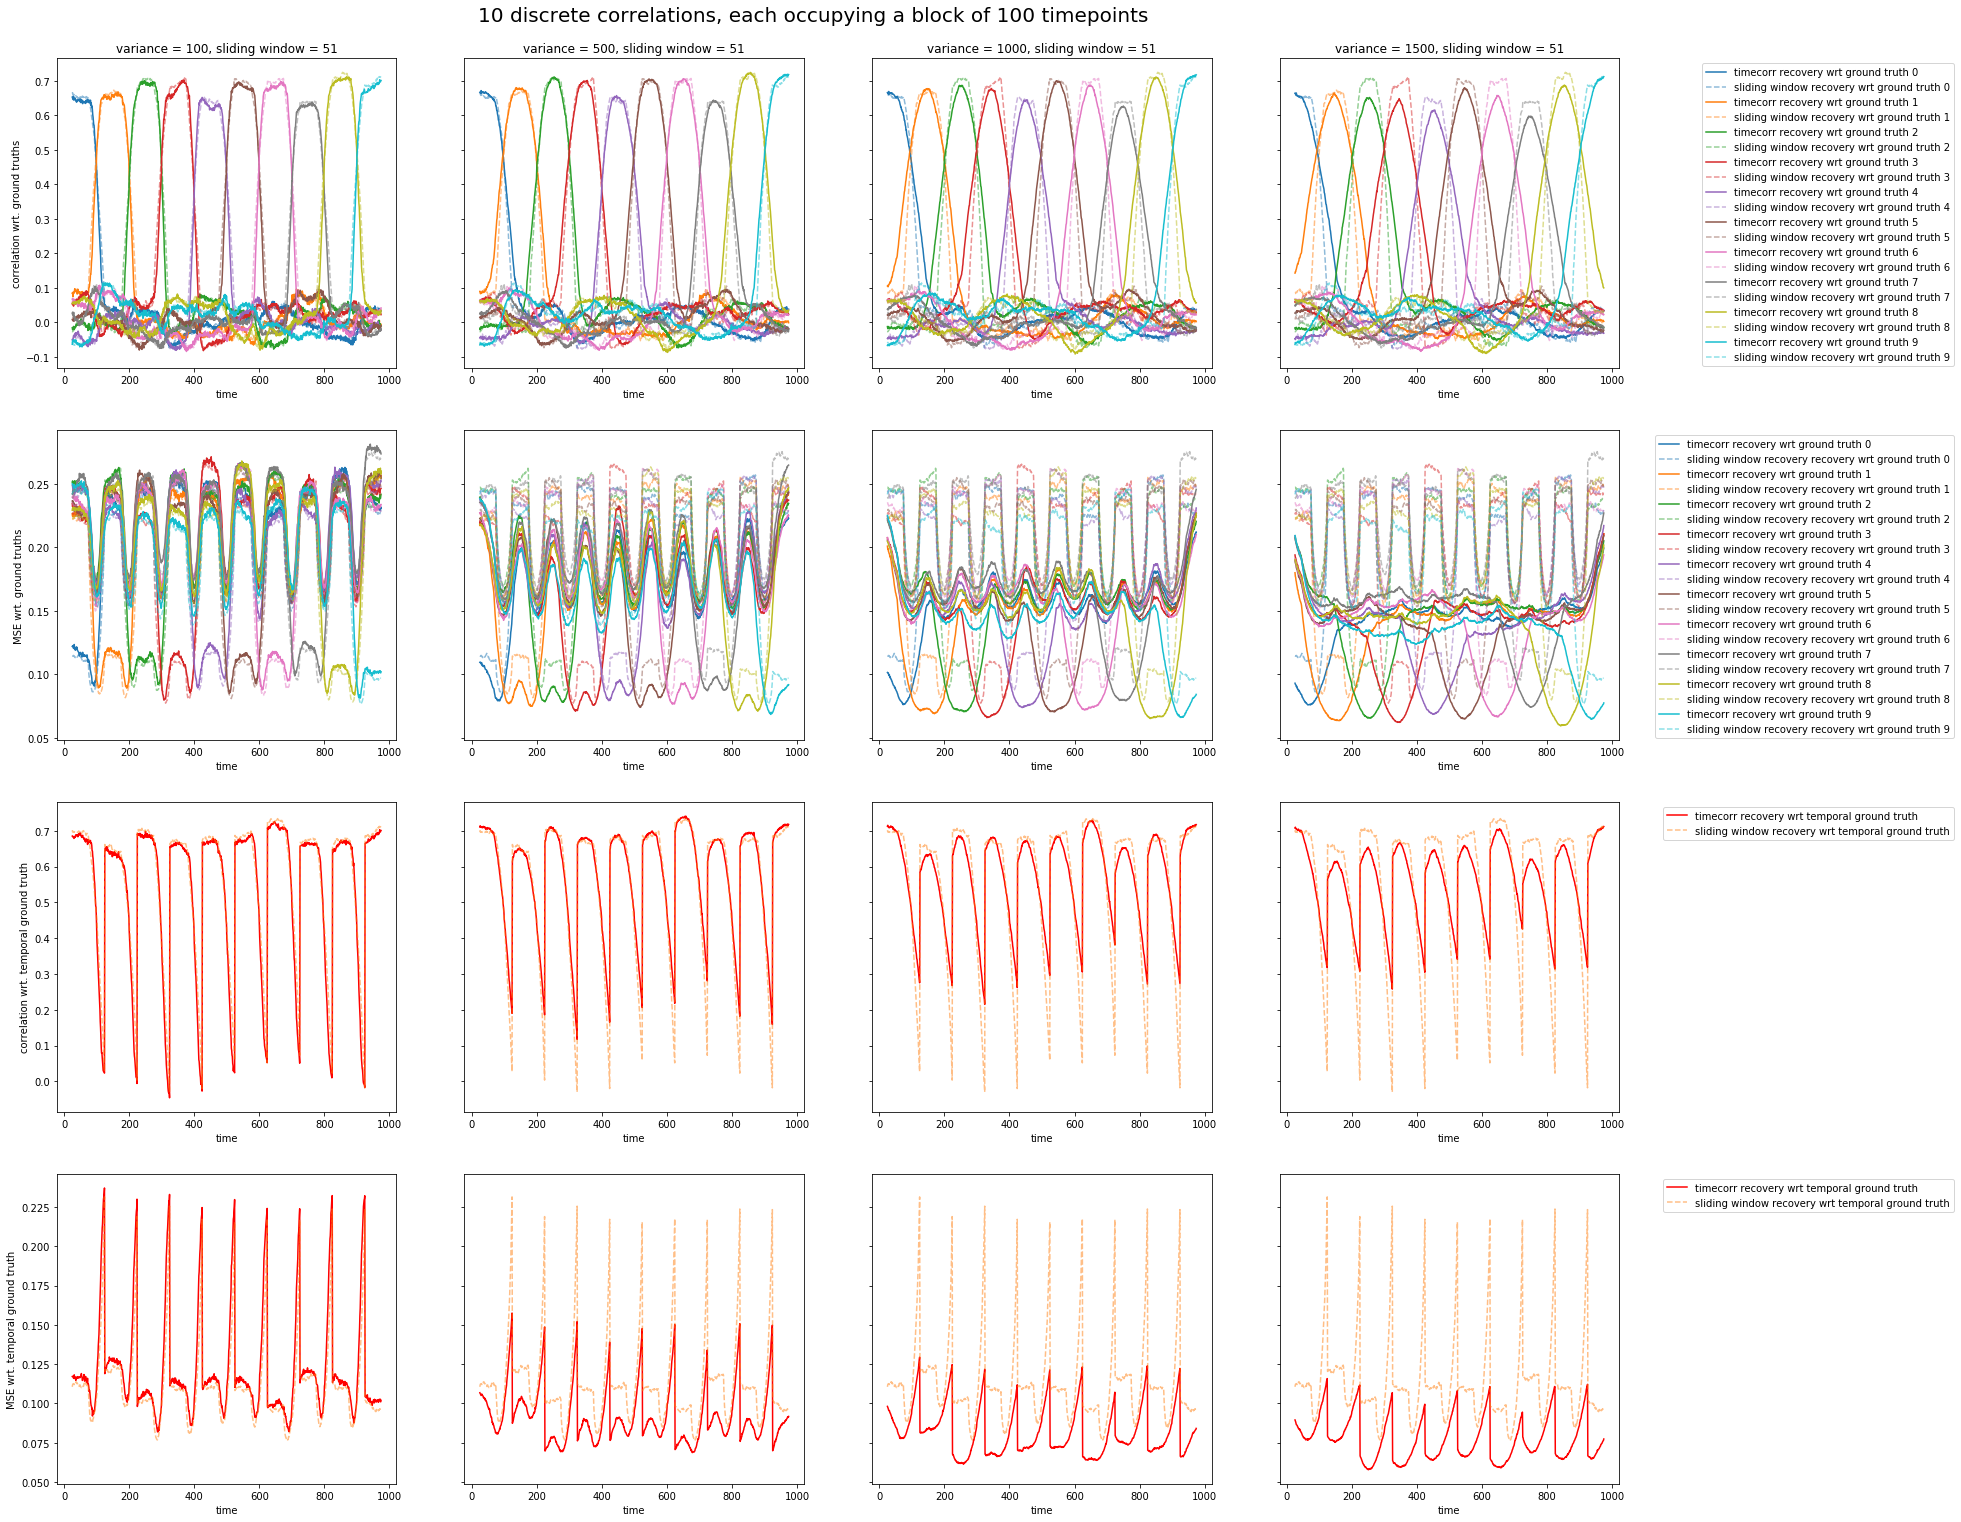
\includegraphics[width=1\textwidth]{../figures/SyntheticTesting/10block100t.png}
\caption{\textbf{Testing on ten 100-time-point blocks, each with different correlations.} In the first row, solid lines show the correlation between block correlations and TimeCorr results; dotted, sliding window results. The different colors represent the correlation between the true correlation in each block and the recovered results (e.g., the blue line represents the correlation between the ground truth in the first block and the recovered results). In the second row, the solid line shows correlation between temporal ground truth and TimeCorr results; dotted, sliding window results. Finally, the columns represent TimeCorr implementations with a different Gaussian variances. The boundaries of each block are indicated by semi-transparent vertical black lines.}
\label{fig:10block100t}
\end{figure}

The graphs displayed in Figure \ref{fig:10block100t} show evaluation of the average results from running TimeCorr and the sliding window method on 100 different block correlation datasets, each containing 10 blocks of 100 time points. The purpose of this dataset is to test how well TimeCorr recovers dynamic correlation structures that rapidly and abruptly changes between different states. The graphs in the first row show that the correlation between the recovered results and the ground truth of a time block peaks within the time span of the time block, but falls to zero at other time points. This result indicates that both the TimeCorr and the sliding window approach are able to easily differentiate the true correlation structure within a block from the true correlation of other blocks. In addition, we can see that results from the TimeCorr approach show different levels of locality and stability with different configurations of Gaussian variance. At low Gaussian variance, the TimeCorr results show high correlation with ground truths at time points near the center of each block where the correlation structure remains unchanged, indicating better imitations of the general structures of the true correlation matrices. In contrast, results from TimeCorr setups with high Gaussian variance demonstrates lower correlation at time points where the correlations structure is stable. We hypothesize this difference may be due to the differences in temporal resolution between TimeCorr setups of varying Gaussian variance. As TimeCorr setups with lower Gaussian variance (higher temporal resolution) place more emphasis on time points closer to the time point of interest and neglect time points further away, their temporal results are less easily influenced by later changes in correlation structures.

The graphs in the second row show the correlation between the temporal ground truth (true correlation at each time point) and the TimeCorr and sliding window results, represented by solid and dotted lines, respectively. As the Gaussian variance of TimeCorr increases, we observe big improvements in the correlation between its results and the temporal ground truths at block borders, where there are abrupt changes in the temporal correlation structure. At time points where the correlation structure is stable and unchanging (block centers), results from TimeCorr setups with low variance demonstrate high correlation with the temporal ground truths, which is consistent with the patterns in the graphs in the first row. These patterns confirm our earlier hypothesis that high resolution (low variance) TimeCorr setups demonstrates better performance when the correlation structure is stable, but TimeCorr setups with low resolution (high variance) is able to recover changing correlation patterns with better accuracy. The performance difference between high Gaussian variance and low Gaussian variance TimeCorr setups also demonstrates that utilization of information from a larger neighborhood of time points is conducive to more effective recovery of dynamically changing correlation structures, while concentrating on a smaller neighborhood of time points gives better recovery of stable correlation patterns.

Finally, the graphs show that the sliding window results are missing information for a number of time points at each end of the time series. As mentioned before, because the sliding window approach requires a sizable buffer for correlation calculation, it is unable to make calculations at the ends of the time series. This loss in information is not very obvious in this synthetic dataset as the sliding window length is very short when compared with the time length of the dataset. However, in other synthetic datasets and real datasets with shorter time lengths, the information loss because more significant and noticeable.

\begin{figure}[!htb]
\includegraphics[width=1\textwidth]{../figures/SyntheticTesting/2block50t4var4slideEB.png}
\caption{\textbf{Testing on two 50-time-point blocks, each with different correlations.} In the first row, the graph on the left shows the correlation (with error bars) between block correlations and TimeCorr results; right, sliding window results. In the second row, the graph on the left shows correlation (with error bars) between temporal ground truth and TimeCorr results; right, sliding window results. Different colors represent different TimeCorr and sliding window implementations.}
\label{fig:2block50t}
\end{figure}

To further confirm our results, we reran the tests on 100 different datasets containing 2 time blocks with different correlations, each spanning 50 time points. Evaluation of the average results from the TimeCorr and the sliding window implementations are shown in Figure \ref{fig:2block50t}, with behaviors of the ground truth displayed for comparison. From these graphs, we can confirm that TimeCorr with low Gaussian variance is able to maintain high correlation with the temporal ground truth at time points where the correlation remains unchanged. In contrast, TimeCorr with low resolution (high Gaussian variance) is able to produce slightly higher correlation and lower MSE across most time points. However, low resolution (high variance) TimeCorr predicts and reacts to future changes in temporal correlation with greater sensitivity, which results in premature changes in its results before the changes in ground truth actually take place.

When looking at the sliding window results, we notice that implementations with longer window length is generally able to produce better recovery results (higher correlation with ground truth). However, longer window length also results in greater data loss, as shown by the gradual decrease in recoverable time span in the sliding window results. In contrast, TimeCorr is able to generate similar, and sometimes even better, results without the data loss.

To explore how TimeCorr performance varies with respect to the relationship between TimeCorr variance and the time span of each block, we conducted another analysis on 100 different datasets containing 2 time blocks with different correlations, each spanning only 11 time points. Evaluation of the average results from the TimeCorr and the sliding window implementations are shown in Figure \ref{fig:2block11t}. The graphs in this figure show that when the TimeCorr variance is greater than the time length of each block, the recovery capabilities of TimeCorr starts to deteriorate. Intuitively, the best way to calculate the correlation within a time block is to only use the time points within the block. Therefore, when the variance is too great, TimeCorr calculations place more weights on time points outside the time block, resulting in deviation from the correct temporal correlation structure. Furthermore, we notice that the TimeCorr setup that generated the best results is the one with variance roughly equal to the length of the time block. This result indirectly tells us that, if a dataset displays similar dynamic correlation structures as the block correlation synthetic datasets, we can extrapolate the lengths of the time blocks in the time series by conducting a cross-validation analysis across TimeCorr implementations with different variances.

In conclusion, as low Gaussian variance (high temporal resolution) TimeCorr implementations can achieve accurate and stable recovery of correlation structures that remain constant over extended blocks of time points and only suffer marginal accuracy loss at abrupt correlation shifts, it is more suitable for fMRI datasets where the dynamic correlation structures of brain activities are similar to that of the block correlation synthetic datasets. In addition, when compared with the sliding window approach, high resolution TimeCorr implementations also boast slightly better recovery performance in general with the additional advantage of no information loss.

\begin{figure}[!htb]
\includegraphics[width=1\textwidth]{../figures/SyntheticTesting/2block11t3var3slideEB.png}
\caption{\textbf{Testing on two 11-time-point blocks, each with different correlations.} In the first row, the graph on the left shows the correlation (with error bars) between block correlations and TimeCorr results; right, sliding window results. In the second row, the graph on the left shows correlation (with error bars) between temporal ground truth and TimeCorr results; right, sliding window results. Different colors represent different TimeCorr and sliding window implementations.}
\label{fig:2block11t}
\end{figure}

\subsubsection{Single Subject Synthetic Dataset with ramping correlations}

In these datasets, we adopt a correlation structure that linearly changes from one terminal correlation $C_1$ to another terminal correlation $C_2$. These datasets will be used to test TimeCorr's ability to accurately recover correlation structures that are dynamically changing over time. To generate a ramping correlation dataset:
\begin{enumerate}
\item Using random normal distribution, generate a dataset X of dimensions $T$ by $V$, where $T$ and $V$ represent the desired time length and voxel (brain region) count, respectively.
\item Generate two terminal correlation matrices $C_1$ and $C_2$, then generate temporal correlation structures at time point $t$ using the function
\begin{align*}
C_t = I\left(\frac{(T-t) \cdot F(C_1)}{T} + \frac{t\cdot F(C_2)}{T}\right)
\end{align*}
where T is the total time length of the datase. $F(x)$ and $I(x)$ represent Fisher Z-transformation and inverse Fisher Z-transformation, respectively. These transformations were applied to ensure stable combination of correlation structures.
\item For activations $X_t$ at each time point in X, transform the data into correlated structure using the Cholesky transformation $C(x)$:
\begin{align*}
W_t = C(C_t) \cdot X_t
\end{align*}
\item Piece everything together to form the new synthetic dataset W that possesses the designated dynamic correlation structure.
\end{enumerate}

To evaluate and compare the performances of TimeCorr and the sliding window method in recovering the ground truth in ramping correlation datasets, we used four metrics: (1) correlation with the two terminal ground truths, and (2) correlation with the temporal ground truth. The first metric was chosen to demonstrate how well TimeCorr and the sliding window method can recover the pattern of linear transition between the two terminal ground truths. The second metric was chosen to demonstrate the overall performance of TimeCorr and the sliding window approach in recovering the temporal ground truth.

\begin{figure}[!htb]
\includegraphics[width=1\textwidth]{../figures/SyntheticTesting/ramp1000t6var6slideEB.png}
\caption{\textbf{Testing different TimeCorr setups on 1000-timepoint ramping datasets.} In the first row, the graph on the left shows the correlation (with error bars) between ground truths at end points and TimeCorr results; right, sliding window results. In the second row, the graph on the left shows correlation (with error bars) between temporal ground truth and TimeCorr results; right, sliding window results. Different colors represent different TimeCorr and sliding window implementations.}
\label{fig:ramp1000t4var}
\end{figure}

First, 100 ramping datasets with 1000 time points were generated to compare how TimeCorr and the sliding window method perform on dynamic correlation structures that gradually linear transitions between two distinct correlation structures. Evaluation of the average testing results are displayed in Figure \ref{fig:ramp1000t4var}. Both methods were able to accurately recover the linear transition patterns between the two terminal ground truth (correlation improves with respect to one terminal correlation but decreases with respect to the other terminal correlation, forming an obvious cross shape). However, as the Gaussian variance of TimeCorr increased, we observe overall improvements in the correlation between the TimeCorr results and the temporal ground truths. This phenomenon is consistent with the patterns we observed in our block correlation synthetic dataset test results, where TimeCorr setups with high Gaussian variance is able to recover dynamically changing correlation structures with much higher accuracy than low variance TimeCorr implementations. However, when we increased TimeCorr's Gaussian variance beyond the time length of the dataset (1000 time points), we saw marginal improvements in TimeCorr's recovery performances. We hypothesize that because all the time points in the time series are already effectively utilized by TimeCorr when the Gaussian variance is equal to the time length of the dataset, increasing the Guassian variance further will have little to no effect on TimeCorr's result.


\begin{figure}[!htb]
\includegraphics[width=1\textwidth]{../figures/SyntheticTesting/ramp500t5var5slideEB.png}
\caption{\textbf{Testing different TimeCorr setups on 500-time-point ramping datasets.} In the first row, the graph on the left shows the correlation (with error bars) between ground truths at end points and TimeCorr results; right, sliding window results. In the second row, the graph on the left shows correlation (with error bars) between temporal ground truth and TimeCorr results; right, sliding window results. Different colors represent different TimeCorr and sliding window implementations.}
\label{fig:ramp500t4var}
\end{figure}

The performance advantage of low resolution (high variance) TimeCorr setups on recovering dynamically changing correlation structures is further verified by the results from testing on 100 ramping datasets of 500 time points. As the temporal correlation linearly transitions between the two terminal correlations within only 500 time points, the average rate of change at each time point is much greater than that of the 1000 time point dataset. Evaluation of the average testing results are displayed in Figure \ref{fig:ramp500t4var}. In contrast to the results from the 1000 time point dataset, the performance difference between different resolution TimeCorr implementations is more evident in the results from the 500 time point datasets. When the Gaussian variance of TimeCorr is increased from 10 time points to 500 time points and beyond, we observe greater improvements in TimeCorr's performance than in the results from the 1000 time point ramping dataset. This pattern confirms the advantage of incorporating information from a wider neighborhood of time points in the recovery of dynamically changing correlations structures. However, when we increased TimeCorr's Gaussian variance beyond the time length of the dataset (500 time points), we saw marginal improvements in TimeCorr's recovery performances. This result confirms our earlier hypothesis that TimeCorr setups with variance equal to dataset time length gives the most optimal performance on datasets with ramping correlation structures.


\begin{figure}[!htb]
\includegraphics[width=1\textwidth]{../figures/SyntheticTesting/ramp100t4var4slideEB.png}
\caption{\textbf{Testing different TimeCorr setups on 100-time-point ramping datasets.} In the first row, the graph on the left shows the correlation (with error bars) between ground truths at end points and TimeCorr results; right, sliding window results. In the second row, the graph on the left shows correlation (with error bars) between temporal ground truth and TimeCorr results; right, sliding window results. Different colors represent different TimeCorr and sliding window implementations.}
\label{fig:ramp100t4var}
\end{figure}

To further explore the characteristics of different resolution TimeCorr setups in recovering highly dynamic correlation structures, we conducted analysis on 100 ramping datasets of only 100 time points, where the linear transitions between the two distinct terminal correlation structures are further accelerated from the 500 time point datasets. Evaluation of the average testing results are displayed in Figure \ref{fig:ramp100t4var}, and confirm our hypothesis from the previous tests: the performance of TimeCorr bottlenecks when its Gaussian variance approaches the time length of the dataset. As the Gaussian of variance of TimeCorr exceeds the total time length of 100 time points, we start to see the cross pattern deteriorate in the first row, indicating worse recovery.

Finally, summarizing the patterns observed from the test results across the 1000-time-point, 500-time-point and 100-time-point datasets, we conclude that high Gaussian variance (low resolution) TimeCorr setups are advantageous in recovering continuously changing correlation structures. In addition, low resolution TimeCorr implementations show optimal performance when its Gaussian variance is equal to the total time length of the dataset. Thus, if the correlation dynamics of an fMRI dataset shows continuous change instead stable blocks, it is most advantageous to use a TimeCorr setup with a Gaussian variance equal the lesser between the total time length and 1000 time points for recovery of its dynamic correlation structure.

Testing results from all three ramping synthetic datasets also demonstrate that the performance of sliding window generally increases as the window length increases, but the rate of improvement decreases dramatically at implementations with longer window length (marginal improvement when the window length approaches $50\%$ of the dataset time length). Although the correlation between the sliding window result and temporal ground truths gradually nears the performance of the optimal TimeCorr implementations as the window length increases, longer sliding window length also results in more significant data loss. In some cases, in order for the sliding window method to reach the same level of performance as TimeCorr, information on more than $50\%$ of the time points in the time series are lost. This tradeoff is highly impractical. Therefore, as TimeCorr is lossless, more flexibly and generally gives better performance, it is more advantageous to use TimeCorr to calculate dynamic functional connectivities of the brain.

\subsection{Testing Inter-Subject Functional Connectivity using TimeCorr}
Confident with TimeCorr's ability to recover the dynamic correlation structures of single subject datasets, we proceeded to test TimeCorr's performance in recovering inter-subject functional connectivity (ISFC) in multi-subject synthetic datasets. In practical scenarios, fMRI datasets always contain a significant amount of noise from non stimulus-driven neural activities. Therefore, to simulate realistic human brain activities, we added different levels of random noise to the synthetic datasets to gauge the robustness of TimeCorr ISFC in recovering stimulus-related functional connectivity. The noise levels we experimented with were on the order of magnitudes of $10\%$ (0.1), $100\%$(1) and $1000\%$(10) of the average activation magnitude. Evaluation of results from running TimeCorr (with Gaussian variance of 300 time points) and the sliding window method (with window length of 101 time points) on 300 ramping datasets (100 datasets for each level of noise), each containing 300 time points, are demonstrated in Figure \ref{fig:t300slide25var1000}.

\begin{figure}[!htb]
\includegraphics[width=1\textwidth]{../figures/ISFC/ramp300t300var101slideEB.png}
\caption{\textbf{Testing ISFC on 300-time-point ramping datasets with different noise levels.} In the first row, the graph on the left shows the correlation (with error bars) between ground truths at end points and TimeCorr results; right, sliding window results. In the second row, the graph on the left shows correlation (with error bars) between temporal ground truth and TimeCorr results; right, sliding window results. Different colors represent different level of noises.}
\label{fig:t300slide25var1000}
\end{figure}

The graphs show that TimeCorr is able to retrieve stimulus-driven dynamic correlation structures with relatively high accuracy at low (0.1) to medium (1) noise levels, but fails to recover any meaningful information when the noise level is too high (10). These results highlight the difficulty of recovering stimulus-driven correlation structures when the subjects display weak cognitive response to the stimulus. However, when the stimuli is able to evoke reasonably strong cognitive response from the subject, TimeCorr ISFC can effectively recover the stimuli-driven dynamic correlation structures with relatively high accuracy.

In addition, even though there is only a limited number of time points in the dataset (300 time points), we chose to use a sliding window setup with a window length of 101 time points to optimize its results. However, even with more than $30\%$ data loss, the sliding window method's performance still barely matches that of TimeCorr. This contrasts further consolidate the advantages of TimeCorr in producing lossless, more stable and accurate recovery of dynamic correlation structures, making it the superior choice for dynamic functional connectivity calculations.

\begin{figure}
\includegraphics[width=1\textwidth]{../figures/ISFC/2block150tslide101var150EB.png}
\caption{\textbf{Testing ISFC on 300-time-point block datasets with different noise levels.} Each time block contains 150 time points. In the first row, the graph on the left shows the correlation (with error bars) between ground truths at end points and TimeCorr results; right, sliding window results. In the second row, the graph on the left shows correlation (with error bars) between temporal ground truth and TimeCorr results; right, sliding window results. Different colors represent different level of noises.}
\label{fig:2block150tslide101var150EB}
\end{figure}

To test how TimeCorr ISFC performs on datasets with abruptly changing dynamic correlation structures, we ran TimeCorr (with Gaussian variance of 150 time points) and the sliding window method (with window length of 101 time points) on 300 datasets (100 datasets for each of the 3 noise levels), each containing 2 time blocks of stable correlation structures spanning 150 time points. Evaluation of the average results are demonstrated in Figure \ref{fig:2block150tslide101var150EB}.

Consistent with the results from testing ISFC on the ramping datasets, we see the quality of recovery of both TimeCorr and the sliding window approach deteriorate with increasing noise levels. In addition, we can see from the graphs on the first row that the sliding window approach demonstrates similar performance to the TimeCorr approach, albeit the sliding window results lose important information for around $30\%$ of the time points. In the graphs displaying the correlations between recovered results and the temporal ground truths, we can see the the sliding window results react very early to the abrupt change at the block border, causing its correlation with the temporal ground truth to dip much earlier than the results from TimeCorr. This phenomenon is caused by the flat averaging component in the sliding window method's calculations. As the sliding window approach places equal weights on every time point within its window of calculation, its results are only a low resolution representations of the average correlation within its window. Because TimeCorr utilizes Gaussian coefficients in its recovery of the temporal ground truth, it places more weight on time points close to the Gaussian center, gaining higher temporal resolution and higher temporal accuracy. As a result, we can see that the TimeCorr results in the stable section of the time series experience less influence from the abrupt changes at the borders of the two time blocks.

\subsection{TimeCorr Decoding Analysis on Real Datasets}
The analyses on synthetic datasets demonstrate the advantages of using TimeCorr for the recovery of single-subject functional connectivities and inter-subject functional connectivities (ISFC) from noisy synthetic datasets. For the next step, we conducted TimeCorr Decoding Analysis (TDA) on real datasets to evaluate how much stimulus-driven brain dynamics information is contained within the ISFC of brain activations. Unlike previous tests with synthetic datasets, the ground truths of the dynamic functional connectivities in actual fMRI datasets are unknown. Therefore, we used the TDA as a noisy proxy to evaluate the quality of functional connectivity recoveries and the quantity of stimulus-driven information within the ISFC of the datasets. Three TimeCorr setups were implemented---each with Gaussian variances of $\text{min}(500,\text{time length})$ time points, 75 time points, or 10 time point---to comprehensively understand the how the recovered results vary under different temporal resolutions. We also recovered ISFC using three different sliding window configurations---each with sliding window length of 101 time points, 51 time points, or 21 time points---as comparison to highlight the strengths and weaknesses of using TimeCorr. These sliding window lengths were specifically selected to establish a fair comparison between the sliding window approach and TimeCorr. As the sliding window method only uses information from time points within its window of calculation, it has to be the equivalent of 6 times the standard deviation of TimeCorr (a span containing $99.7\%$ of the area under the Gaussian curve), where $99.7\%$ of its temporal weights are contained. Therefore, the following equation is used to calculate the corresponding window length from TimeCorr variance:
\begin{align*}
\text{sliding window length} = 6\sqrt{TimeCorr variance}.
\end{align*}
We did not use the exact values obtained through this equation, but rather used rough approximations that cover ranges of window lengths that could give us a more comprehensive understanding of the variations in sliding window performance.

Three different datasets were used for this analysis: Sherlock, Pieman, and Forrest. Detailed descriptions for each dataset are included in the corresponding subsections. For each dataset, we first used Incremental PCA to reduce the fMRI matrices to only 100 voxels (making the dataset more manageable for large scale calculation), and then conducted 100 repetitions of the TimeCorr Decoding Analysis, each with different random group divisions, on the reduced activations. The results displayed below are the average of 100 repetitions.

\subsubsection{Description for the Pieman Dataset}
This dataset was collected by Uri Hasson's lab in 2016 \citep{hasson2016}. The stimuli for this experiment were derived from a 7 minute recording of the ``Pie Man" story by Jim O'Grady. The experimental subjects were all native English speakers with normal hearing. Four testing conditions with random subject assignments were implemented: 36 subjects listened to the story from beginning to end, and were labelled as the ``intact" group; 18 subjects listened to a version of the story where the paragraphs were scrambled randomly, and were labelled as the ``paragraph" group; 36 subjects listened to a version of the story where the words were scrambled randomly, and were labelled as the ``word" group; lastly, 36 subjects did not listen to anything and stayed in resting state throughout the experiment, and were labelled as the ``resting" group. 12 seconds of neutral music and 3 seconds of silence preceded and 15 seconds of silence followed each playback in all conditions. The brain activities of all subjects for the duration of the experiment were recorded into fMRI datasets, with the data from music and silence periods discarded from all analyses.

\subsubsection{Description for the Forrest Dataset}
This dataset was collected by Michael Hanke and colleagues in 2014\citep{Hanke2014}. The stimuli for this experiment is a two-hour presentation of an audio-only version of the Hollywood feature film ``Forrest Gump", which was made specifically for a visually impaired audience. The movie was divided into eight 15-minute sessions with breaks in-between, and presented to 20 subjects with normal hearing. During each session, brain activities centered on the auditory cortices in both brain hemisphere and the frontal and posterior portions of the brain were recorded into high resolution 7-Tesla fMRI datasets.

\subsubsection{Description for the Sherlock Dataset}
This dataset was collected by Uri Hasson's Lab in 2017 \citep{Chen2017}. Sixteen participants (17 were described in the original paper, but one was removed from this dataset due to a small amount of missing data at the end of the movie scan) were presented with a 50-minute segment of the audio-visual movie Sherlock (BBC) while undergoing fMRI scan. Following the movie, participants were asked to describe, without any external guidance, what they recalled of its content in as much detail as they could while undergoing brain imaging. Participants were allowed to speak on any aspect of the movie for as long as they wished, while their speech was recorded with an fMRI-compatible microphone.

\subsubsection{Results}


\begin{figure}[!htb]
\includegraphics[width=1\textwidth]{../figures/CircularAnalysis/intact.png}
\caption{\textbf{TimeCorr Decoding Analysis on the Pieman ``intact" dataset} Moment by moment correlation (with error bars) between the ISFC of two equal subdivisions of subject data. The graph on the left represent the decoding results using ISFC calculated using different TimeCorr configurations. The graph on the right represent the decoding results using ISFC calculated using different sliding window configurations.}
\label{fig:intact}
\end{figure}

The results from running the TimeCorr Decoding Analysis (TDA) on the Pieman ``intact" dataset is displayed in Figure \ref{fig:intact}. At first glance, we noticed that the general range of correlation values obtained through the TDA is much lower than that of our synthetic dataset testing results. This indicates that there is a lot of noise from non stimulus-driven brain activities.

In addition, we noticed that TimeCorr implementations with different variances display very different correlation curves. The TDA results from ISFC calculated using TimeCorr with high variance (300 time points) has a smoother correlation curve that generally contains relatively higher correlation values across all time points. In contrast, the low variance TimeCorr (10 time points) results generally consists of lower correlation values, but also contains occasional peaks with correlation values exceeding the values from high variance TimeCorr results. This difference indicates that the dynamic correlation structure in the time series is a mixture of both the ramping and the block structures from our synthetic testing. Time blocks with stable correlation structure appears occasionally throughout the time series, but the correlation dynamics in between blocks resemble that of gradual change (ramping synethetic datasets). Using the conclusions from testing on synthetic datasets, we can extrapolate that low variance TimeCorr produced a better recovery of the functional connectivities of time point within the block structures and high variance TimeCorr performed better on the linear transitions in between time blocks.

Furthermore, we observe that the location and height of the peaking structures in TimeCorr results is also reproduced in the sliding window results. Knowing that high correlation is an indication of similar behavior across all subjects and taking into consideration that the curves are results from averaging over 100 repetitions, a process that cancels out most random noise, we can conclude with confidence that these patterns are realistic representations of inter-subject functional connectivities of stimulus-driven brain activities.

Lastly, we noticed that the peaks in TimeCorr results were slightly higher than those in the results from sliding window. This difference can be attributed to TimeCorr's flexible ability to change between different temporal resolutions. With lower Gaussian variance, TimeCorr has higher temporal resolution and is able to produce a more accurate recovery of the temporal activities at a time point. In comparison, because the sliding window uses flat averaging, the peaks are partially canceled out by the lower values of the surrounding time points, resulting in a lower value.

\begin{figure}[!htb]
\includegraphics[width=1\textwidth]{../figures/CircularAnalysis/paragraph.png}
\caption{\textbf{TimeCorr Decoding Analysis on the Pieman ``paragraph" dataset} Moment by moment correlation (with error bars) between the ISFC of two equal subdivisions of subject data. The graph on the left represent the decoding results using ISFC calculated using different TimeCorr configurations. The graph on the right represent the decoding results using ISFC calculated using different sliding window configurations.}
\label{fig:paragraph}
\end{figure}

The TDA results on the Pieman ``paragraph" dataset is displayed in Figure \ref{fig:paragraph}.
Overall, the curves for every TimeCorr and sliding window setups demonstrates lower correlation values when compared with that of the Pieman ``intact" dataset. This difference can be explained by a decrease in the coherency of the stimuli---from an intact story to out of order paragraphs---which intuitively would invoke weaker brain responses from the subjects. In addition, when compared with the sliding window results, TimeCorr's correlation curves contains higher peaks. This is consistent with the patterns in the results from the Pieman ``intact" dataset, where TimeCorr is able to achieve better recovery of the stimulus-driven activities blocks due to its ability to reach higher temporal resolution. Lastly, we observe that the sliding window results contain significant data loss (missing time points at each end of the time series) while only producing similar and often times lower decoding correlation than TimeCorr results.

\begin{figure}[!htb]
\includegraphics[width=1\textwidth]{../figures/CircularAnalysis/word.png}
\caption{\textbf{TimeCorr Decoding Analysis on the Pieman ``word" dataset} Moment by moment correlation (with error bars) between the ISFC of two equal subdivisions of subject data. The graph on the left represent the decoding results using ISFC calculated using different TimeCorr configurations. The graph on the right represent the decoding results using ISFC calculated using different sliding window configurations.}
\label{fig:word}
\end{figure}

The results of the Pieman ``word" dataset, displayed in Figure \ref{fig:word}, displays similar patterns to that of the Pieman ``paragraph" dataset. However, we notice that the correlation peaks/blocks are generally lower in the Pieman ``word" time series, which is suggestive of weaker subject brain response (similar to the difference between ``intact" and ``paragraph"). We also noticed that the results from the Pieman ``word" dataset has a slightly lower resampling accuracy than both the ``intact" and the ``paragraph" dataset, meaning that the activities at sequential time points in the ``word" times series display higher similarity with each other. Both of these contrasts confirms that the stimuli under the ``word" condition---random arrangements of words that have no coherent meaning---was not able to generate very salient responses from the subjects.

\begin{figure}[!htb]
\includegraphics[width=1\textwidth]{../figures/CircularAnalysis/resting.png}
\caption{\textbf{TimeCorr Decoding Analysis on the Pieman ``resting" dataset} Moment by moment correlation (with error bars) between the ISFC of two equal subdivisions of subject data. The graph on the left represent the decoding results using ISFC calculated using different TimeCorr configurations. The graph on the right represent the decoding results using ISFC calculated using different sliding window configurations.}
\label{fig:resting}
\end{figure}

The correlation curves for the Pieman ``resting" dataset, as displayed in Figure \ref{fig:resting}, almost all fall to 0 at the start of the time series. This phenomenon suggests that there is almost no similarity between the subject responses throughout the time series. In addition, we observe that the resampling accuracy of the Pieman ``resting" dataset is only half of that of the other Pieman datasets, meaning that there is barely any difference in activities between sequential time points. As the subjects remained in resting state throughout the duration of this dataset, there is no common stimuli between the subjects, therefore brain activity patterns should remain stable throughout each subject's time series but differ greatly between subjects. These different brain responses causes the corresponding ISFC to contain little to no meaningful information, thus resulting in correlation values of 0 throughout the time series.

In summary, when comparing between the TDA results of different Pieman datasets (``intact", ``paragraph", ``word", ``resting"), we can see that as the complexity and integrity of the stimulus decreases, the decoding correlation decreases in general. This makes sense as the human brain should intuitively produce more potent cognitive response to more coherent and meaningful stimuli (intact), weaker response to scrambled and irrational stimuli (paragraph, word), and little to no response to no stimuli (resting). In addition, due to the application of Gaussian averaging in its calculations, TimeCorr is able to reach higher temporal resolution than the sliding window method and achieve better recovery of the functional connectivity dynamics at time points with peaking decoding correlation. Lastly, unlike the sliding window method, TimeCorr results does not have data loss, which directly translates to more useful information being recovered, more flexibility in the selection of its Gaussian variance and the ability to recover greater variety of dynamic correlation structures.

\begin{figure}[!htb]
\includegraphics[width=1\textwidth]{../figures/CircularAnalysis/forrest.png}
\caption{\textbf{TimeCorr Decoding Analysis on the Forrest dataset} Moment by moment correlation (with error bars) between the ISFC of two equal subdivisions of subject data. The graph on the left represent the decoding results using ISFC calculated using different TimeCorr configurations. The graph on the right represent the decoding results using ISFC calculated using different sliding window configurations.}
\label{fig:forrest}
\end{figure}

The results from both the Forrest dataset and the Sherlock dataset, shown in Figure \ref{fig:forrest} and Figure \ref{fig:sherlock}, respectively, show very similar patterns as the results from the Pieman ``intact" dataset. Overall, their decoding correlation curves are much lower than that of synthetic datasets, indicating that a lot of non stimulus-driven activities exist in the dataset. In addition, we observe that the correlation structures recovered by high resolution (low variance) TimeCorr displays rapid and sharp fluctuations. In contrast, the correlation curves from the sliding window methods are much smoother with less distinction in their structure. Furthermore, as the Gaussian variance of TimeCorr increases (lower temporal resolution), we observe that the small peaks are smoothed and combined into wider and higher peaks that start to resemble the correlation structure of synthetic block correlation datasets, albeit the blocks in the Forrest dataset and the Sherlock dataset each has different time spans. However, when we increase the effect of averaging in the sliding window approach by increasing the sliding window length, we observe the preivously distinct structures start flatten and conform to the neighboring time points. Overall, in comparison with the results from the sliding window approach, the TimeCorr results contains more salient peak responses with more distinct borders, indicating higher temporal resolution and more accurate representation of the moment to moment dynamic functional connectivity.


\begin{figure}[!htb]
\includegraphics[width=1\textwidth]{../figures/CircularAnalysis/sherlock.png}
\caption{\textbf{TimeCorr Decoding Analysis on the Sherlock dataset} Moment by moment correlation (with error bars) between the ISFC of two equal subdivisions of subject data. The graph on the left represent the decoding results using ISFC calculated using different TimeCorr configurations. The graph on the right represent the decoding results using ISFC calculated using different sliding window configurations.}
\label{fig:sherlock}
\end{figure}


To summarize, the decoding correlation curves across all TimeCorr and sliding window setups for all real fMRI datasets are generally much lower than that of the synthetic datasets in prior tests. The overall decrease in moment-by-moment decoding correlation strongly indicates that a lot of noise created by non stimulus-driven brain activities exists within these datasets. Furthermore, the correlation curves from high resolution TimeCorr recoveries contains distinct peak/block structures, while the correlation curve from low resolution TimeCorr recoveries show smooth transitions in-between successive peaks. This difference suggests that the dynamic correlation structures in actual datasets contain a mixture of block correlation structures with linear transitioning in-between.

Another important factor that causes smoothing in the time series is the coherency of the stimuli. From the results of the Pieman dataset, we observe higher and more distinct peaks in results of the ``intact" and ``paragraph" datasets, and smoother and lower correlation curves in the results of the  ``word" and ``resting" dataset. This shows that potent and coherent stimuli is able to stimulate stronger and more distinctive brain activities, while weak and incoherent stimuli fails to evoke any meaningful response from the brain.

When comparing between the results from the sliding window approach and TimeCorr, we notice that the structures in TimeCorr results are more distinctive (e.g., sharper and higher peaks), which can be attributed to TimeCorr's high temporal resolution from the usage of Gaussian distribution. As we decrease the resolution (increase the Gaussian variance) of TimeCorr, we observe a smoothing effect over the correlation curve. However, because TimeCorr uses Gaussian averaging instead of flat averaging, it is able to preserve important patterns in the dataset even at low resolutions. In comparison, because the sliding window method uses flat averaging in its calculations, increasing the window length causes salient correlation structures throughout the time series to be flattened and blended into surrounding time points.

Lastly, we observe that the results from the sliding window method contains significant data loss, which can sometimes equate to $30\%$ of the total time points in a dataset. In contrast, TimeCorr possesses higher flexibility and temporal resolution, and is able to preserve the integrity of the time series while producing similar and often times better quality of recovery. In conclusion, we believe that TimeCorr is the more preferable method of dynamic functional connectivity calculations.


\clearpage
\newpage
\section{Conclusion}
We proposed TimeCorr, a lossless and high resolution alternative to the sliding window approach for functional connectivity calculation, and TimeCorr Decoding analysis, a new means of evaluating the quality of functional connectivity recovery from actual fMRI datasets. Through testing on synthetic data, we demonstrated the superiority of the TimeCorr approach over the sliding window approach in recovering dynamic functional connectivities, as well as its ability to differentiate between datasets with different correlation dynamics (block vs ramping). Then, to understand how well TimeCorr and the sliding window method compares in recovering stimulus-driven brain dynamics information from fMRI data, we carried out TimeCorr Decoding Analysis on three real fMRI datasets using different configurations (temporal resolutions) of TimeCorr and the sliding window method. Finally, from the patterns displayed by the correlation curves in the results of our TimeCorr Decoding Analysis, we used our conclusions from synthetic dataset testing to extrapolate that the brain activities in the Pieman, Sherlock and Forrest datasets may consist of a mixture of multiple different length time blocks, each possessing stable correlation structures within its scope, with linear transition in-between. Christopher Baldassano and colleagues confirmed this extrapolation for the Pieman and the Sherlock datasets in one of their recent papers \citep{Baldassano2016}.

From our tests on the Pieman, Sherlock and Forrest datasets, we saw that the TimeCorr's flexibility in temporal resolution revealed different dynamic functional connectivity patterns subject brain activations. In addition, we were able to visualize, compare and achieve a better understanding of these dynamic patterns through the TimeCorr Decoding Analysis. With more knowledge on the dynamics behind our brain activities, we increase our capability to decode the intricacies behind human perception, learning and growth, and improve the quality of life.

In order to further improve TimeCorr and dynamic functional connectivity research in general, we intend to experiment with the following options:

Firstly, we now have more confidence that the brain activities of subjects in the Pieman, Forrest and Sherlock datasets on average mainly consists of time blocks of stable correlation structures. Therefore, to better calculate the temporal functional connectivity at each time point, using only activations of time points within the scope of the corresponding correlation time block could significantly improve the accuracy of our calculations. One difficulty to this approach is the detection of block borders where the abrupt correlation changes occur. Christopher Baldassano and colleagues have tried using a variant of the Hidden Markov Model to detect the transitions between time blocks and achieved good results \citep{Baldassano2016}. We believe incorporating this approach into our TimeCorr approach could very likely improve the quality of our functional connectivity recoveries.

Secondly, although replacing flat averaging with Gaussian averaging greatly improved the temporal accuracy of our recovery efforts, we feel like there is still room to increase the temporal resolution of our methods. Therefore, we plan to experiment with alternative distributions (e.g. Laplacian Distribution) for TimeCorr coefficients generation to achieve even better temporal accuracy in our recovery of dynamic functional connectivities.

Thirdly, we plan to experiment with other dimensionality reduction algorithms for the initial voxel-wise reduction of fMRI datasets. Although PCA is able to efficiently combine brain voxels with similar activity patterns and effectively preserve the general correlation dynamics within a dataset, it loses considerable amounts of important information by neglecting spatial distinctions between voxels. The correlation between voxels with similar activity patterns may be disposable when the voxels are from the same brain region, but the correlation between similar voxels across different brain regions could potentially contain very important information on the stimulus-driven dynamics of the brain. In addition, the underlying distribution of brain activations does not necessarily follow a normal distribution, which may greatly decrease the effectiveness of PCA in dimensionality reduction of brain data. We believe factor analysis and autoencoder neural networks may prove to be effective alternative methods of dimensionality reduction that is worth exploring.

Lastly, we believe that important information may exist beyond voxel activations and their first level functional connectivities. The brain is a network of seemingly autonomous nodes that are actually intricately interconnected. Intuitively, voxels in the brain are analogous to the intersections within a 3-dimensional web: all voxels are delicately connected with each other, forming small sections that interweave into larger and larger clusters. Similarly, when we find the temporal correlation between two voxels, we gain information on how they interact with each other at that specific time point. By ``leveling up", we find the correlation between the interactions of two pairs of voxels, which gives us additional information on the dynamics of a slightly larger community (4 voxels). Following this intuition, every time a new order of functional connectivity is calculated on top of another level of functional connectivity, we are essentially retrieving information on the dynamic relationship between increasingly larger clusters. Therefore, to fully grasp the functions of a single brain region in the network, it is crucial to understand its activities in the context of the richly woven network that supports it \citep{Battiston2017}. As demonstrated by previous efforts by the Contextual Dynamics Lab, high level functional connectivities may contain non-overlapping cognitive information inaccessible by functional connectivities at lower levels \citep{jeremy2017}. Therefore, incorporating information from higher order dynamics could potentially improve the quality of brain analyses.

To conclude, recovering the dynamic functional connectivity patterns in noisy fMRI datasets is a challenging task, but is also crucial for achieving a more in-depth and comprehensive understanding of stimulus-driven brain dynamics. We introduced the TimeCorr and TimeCorr Decoding Analysis as new means to calculate and examine functional connectivity structures in brain fMRI datasets. Using these methods, we were able to discover important dynamic correlation patterns in the brain that were heretofore inaccessible. We believe the applications and benefits of understanding the dynamic brain functional connectivities are endless, and we are excited to explore new approaches to improve our research methods and expand the horizon of human brain decoding.

\newpage
\bibliographystyle{apalike}
\bibliography{ThesisTHC}
\end{document}
